\chapter[]{Anomaly Detection Using Recurrent Neural Networks}


\section{Introduction}

Chapters \ref{ch:ad} and \ref{ch:rnn}, separately, introduced anomaly detection in time series and recurrent neural networks as time series modelers.
%
This chapter outlines a procedure for finding anomalies using RNNs with the goal of mitigating many of the problems associated with anomaly detection that were discussed in \ref{ch:ad}.
%
As much as possible, the same procedure is applied for each time series used to test the procedure.


The outlines describes:
%
\begin{description}
%
\item[sampling:] the time series used for training and its associated sampling process
%
\item[recurrent autoencoders:] the specific form of the RNN
%
\item[training:] the training algorithm used on the RNN
%
\item[Bayesian optimization:] the search for optimized parameters for the procedure
%
\end{description}

%todo: results or anom data

\section{Sampling: Sliding Windows}
\label{sec:sampling}

Some univariate time series \emph{with} anomalies were chosen or generated to test the anomaly detection process:

\begin{description}

\item[electrocardiogram  (ECG):] a signal from the human heart taken from the PhysioNet \cite{PhysioNet} database.
%todo: ecg data is popular. see why in results.

\item[polysomnography ECG (PSG-ECG):] human ECG data \cite{PhysioNet} taken during a sleep study%
\footnote{University College Dublin Sleep Apnea Database, \url{http://www.physionet.org/physiobank/database/ucddb/}, doi:10.13026/C26C7D, study id. ucddb002}%
.

\item[power demand:] a building's electrical power usage data
\footnote{\url{http://www.cs.ucr.edu/~eamonn/discords/power_data.txt}} referenced in the influencial HOT-SAX paper \cite{Keogh2005} (for anomaly detection in time series).

\item[spike:] a generated sequence that is simply evenly-spaced `spikes' of the same height.

\item[sine:] a generated sinusoidal signal.

\end{description}
\noindent
%
The normal behaviour, as well as anomalous behaviour, of these time series can be seen in the plots presented in Section \ref{sec:results}.%
%todo: along with an explanation of why it was chosen

While there is only one `master' time series to train on (in each test), the RNN needs to see many `samples' from the master time series.
%
The sliding window procedure, described in \ref{sec:adsample}, is used to get samples of some window length.
%
Additionally, since RNNs do not need a fixed window, sliding windows are obtained for more than one window length.
%
Furthermore, the samples are collected into `mini-batches' (of the same window length) to be more compatible with the training procedure.
%
The window length is incremented (size skip) from some minimum until it is not possible to obtain a mini-batch (so the largest window will be close to the length of the time series).


Table \ref{tbl:winspec} specifies the relevent sizes and increments for the sampling process.
%
The values were adjusted manually until a `reasonable' number of samples were found.
%
However, the minimum window length was chosen such that meaningful dynamics were captured (regardless of the scale of the anomaly).

%todo: why extra line ???
\begin{table}[H]
  \centering
  \csvreader[
  % need p b/c the below \ifthenelse 'filters' make the tbl cell ugly
  tabular=|p{.75in}||c|c|c|c|c||c| 
  ,table head=
  \hline
  \bfseries series
  &  length 
  &  min. win.
  &  slide skip 
  &  size skip 
  &  batch size
  &  $\Rightarrow$ \bfseries samples 
  \\ \hline  \hline
  ,late after line=\\\hline
  ]%
  {tbls/sampling.csv}%
  {
    batch_size=\bs
    ,length=\ln
    ,min_winsize=\mw
    ,name=\nm
    ,nsamples=\ns
    ,slide_jump=\ss
    ,winsize_jump=\wss
  }%
  {
    %these act like filters. so you have to explicitly get them
    \ifthenelse{ \equal{\nm}{spike}}{\noindent spike}{}
    \ifthenelse{ \equal{\nm}{sin}}{\noindent sine}{}
    \ifthenelse{ \equal{\nm}{power}}{\noindent power}{}
    \ifthenelse{ \equal{\nm}{ecg}}{\noindent ECG}{}
    \ifthenelse{ \equal{\nm}{sleep}}{\noindent  PSG-ECG}{}

    & \ln & \mw & \ss & \wss & \bs & \ns
  }
\caption[]{Time series sample specifications} %todo: what case?
\label{tbl:winspec}
\end{table}


\section{RNN Setup: Autoencoder}

The RNN needs to learn what normal time series behaviour is.
%
So an autoencoder is used which can learn expected behavior by setting the target, $\vc{y}$, to be the input, $\vc{x}$.
%
The loss function is MSE (Equation \ref{eqn:mse}).
%
Furthermore, to prevent the RNN from learning trivial identity functions, Gaussian noise is added to the input where the standard deviation is equal to .75 the standard deviation of the whole time series.

\begin{equation*}
 \tilde{\x} = \x
 + \mathcal{N}(0,(0.75\sigma_{\mathrm{std}}(\x))^2)
\end{equation*}
\noindent
%
Note the comparison in the loss function is between the (uncorrupted) signal, $\x$, and the output from the network, $\vc{o}$, given $\x$: $L(\vc{o}(\tilde{\x}),\x)$.
%
With this setup, a denoising autoencoder, the data generating process, $p(\x)$, is implictly learned \cite{Bengio2013}.


\section{Training}


SGD with RMSprop \cite{Tieleman2012} for parameter updates has been demonstrated to provide results that are similar to more sophisticated second-order methods but with significantly less computational cost \cite{Dauphin}.
%
Another benefit of RMSprop is that it is designed to work with mini-batch learning.
%
Since the training data is highly redunant (from sliding windows), it is expected that computing the gradient (to update parameters) from a subset of the data (mini-batch) is more efficient than computing the gradient for all the data.


For each derivative in the gradient, RMSprop keeps an exponentially-weighted moving average of derivative magnitudes which normalizes the derivative by its root-mean-squared.
%
More specifically, the (overall) RNN training procedure is outlined in the following box.

\begin{algorithm}{Training Procedure}
\begin{algorithmic}
\STATE \STATE

\STATE \COMMENT{obtain mini-batches (as Section \ref{sec:sampling})}
\STATE $\mathcal{X} \gets \mathrm{sampling}(\x)$
\STATE \STATE

\STATE \COMMENT{randomly split mini-batches into training and validation sets}
\STATE $\mathcal{X}_t \gets \mathrm{choose(75\%,\mathcal{X})}$
\STATE $\mathcal{X}_v \gets \mathcal{X} - \mathcal{X}_t$
\STATE \STATE

\STATE \COMMENT{initalize}
\STATE $\vc{\theta} \gets \vc{0}$
\COMMENT{initial RNN parameters are 0}
\STATE \COMMENT{set training parameters}
\STATE $\alpha = 10^{-4}$
\COMMENT{learning rate}
\STATE $h = 14$
\COMMENT {RMS `halflife'}
\STATE $\gamma \gets e^{\frac{-\ln{2}}{h}}$
\STATE $r = 10^{-8}$
\COMMENT{RMS regularizer}
\STATE patience = 5
\COMMENT{stopping criterion parameter}
\STATE min\_improvement = $.005$
\COMMENT{stopping criterion parameter}
\STATE \STATE

%\STATE $i \gets 1$
\FOR{epoch $i$}
\STATE{ $\mathcal{X}_t \gets  \mathrm{shuffle}(\mathcal{X}_t)$}

\FOR{minibatch $M$ in $\mathcal{X}_t$ }

\FOR{parameter $p$ in $\vc{\theta}$}
\STATE{} \COMMENT{per-parameter, update $p$ according to RMSprop \cite{Graves2013b}
(indices to $p$ omitted)}
\STATE{
  \begin{flalign*}
    f_{i+1}
    &\gets 
    \gamma f_i 
    +
    (1 - \gamma) 
    \frac{\partial{L}}{\partial{p}} && 
    \\
    g_{i+1}
    &\gets
    \gamma g_i
    +
    (1 - \gamma)
    \left(
      \frac{\partial{L}}{\partial{p}}
    \right)^2 && 
    \\
    p_{i+1}
    &\gets 
    p_i
    - 
    \frac{\alpha}{
      \sqrt{g_{t+1} 
        - f_{t+1}^2 
        + r}
    }
    \frac{\partial{L}}{\partial{p}} &&
  \end{flalign*}
}
\ENDFOR
\ENDFOR

\STATE \COMMENT{compute average loss on validation set}
\STATE{
  $
  v_i
  \gets
  \frac{1}{|\mathcal{X}_v|}
  \sum_{\x_v \in \mathcal{X}_v}
  L(\x_v,\vc{o})
  $
}


\STATE \COMMENT{stop when no improvement more than patience times}
\IF{
$v_{min}-v_{i}> v_{min} \cdot \mathrm{min\_improvement}$
}
\STATE{$v_{min} \gets v_i$}
\STATE{$i_{min} \gets i$}
\ENDIF

\IF{$i - i_{min} > \mathrm{patience}$}
\STATE{STOP} \COMMENT{return $\vc{\theta}$}
\ENDIF

\STATE{$i \gets i+1$}
\ENDFOR

%\STATE% \STATE
\end{algorithmic}
\end{algorithm}

%todo: use s=h in lstm

The \texttt{theanets} \cite{Johnson2015} implementation of RNNs and RMSprop
\footnote{With every calculation of $\vc{o}$, the RNN states are initialized to 0.}
was used.
%
\texttt{theanets} is based on the mathematical expression compiler, \texttt{theano} \cite{Bergstra2010}.
%
Gradients were computed using \texttt{theano}'s automatic differentiation feature instead of explicitly-defined backpropagation \cite{Rumelhart1986}.

%\section{Hyper-parameter Optimization}
%In the previous section, 

While the training procedure optimizes $\vc{\theta}$, there are other parameters that could be adjusted to minimize the loss.
%
The number of layers, $l$, and the `size' of each layer, $n$, corresponding the dimension of vector $\vc{s}$ (which equals the cell state mem), were chosen as `hyper-parameters' for optimization in a Bayesian optimization process.
%
Bayesian optimization is suited for optimizing RNN training because
1) it tries to minimize the number of (expensive) objective function calls, which, in this case, is the training procedure, and
2) it considers the stochasticity of the function, which, in this case, the selection of training and validation data are random in addition to the training data shuffling on each epoch.


The \texttt{spearmint} \cite{snoek2012practical} package was used to drive the hyper-parameter optimization process.
%
The process was programmed to save RNN parameters after every optimization iteration.
%
\texttt{spearmint} takes a parameter search space and a maximum number of optimization iterations.
%
However, the process was stopped until the RNN with the minimum validation loss was subjectively able to detect anomalies
%
\footnote{
Further optimization was possible with increasing RNN size but loss reduction diminished relative to the associated increase in computational expense.
}
.


Figure \ref{fig:bo} shows the results of the process.
%
Each point is the average validation loss since more than training session could have been launched with the same parameters.
%
If so, the points have a 95\% confidence interval bar through them.

\begin{figure}[t!]
    \centering
  
  \begin{subfigure}[t]{\textwidth} %hmm it's the same width as the pdf
%todo: check the previous pdfs includegraphics
        \centering
        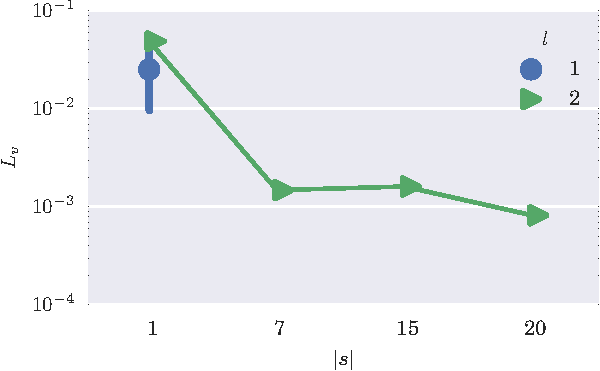
\includegraphics[]{figs/bo_spike.pdf}
        \caption{spike}
    \end{subfigure}%
  
    \begin{subfigure}[t]{\textwidth}
        \centering
        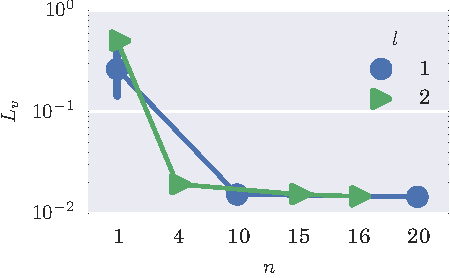
\includegraphics[]{figs/bo_sin.pdf}
        \caption{sine}
    \end{subfigure}%

    \begin{subfigure}[t]{\textwidth} 
        \centering
        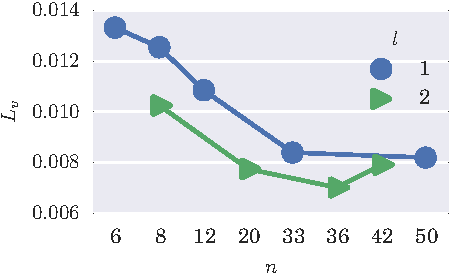
\includegraphics[]{figs/bo_power.pdf}
        \caption{power}
    \end{subfigure}%

\end{figure}
\begin{figure}
    \ContinuedFloat %3 figs a pg

    \begin{subfigure}[t]{\textwidth} 
        \centering
        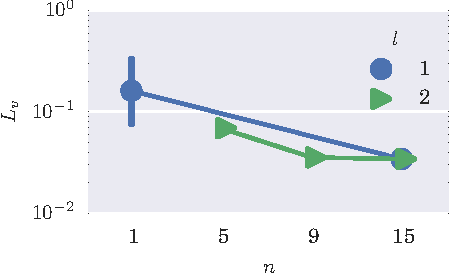
\includegraphics[]{figs/bo_ecg.pdf}
        \caption{ECG}
    \end{subfigure}%

    \begin{subfigure}[t]{\textwidth} 
        \centering
        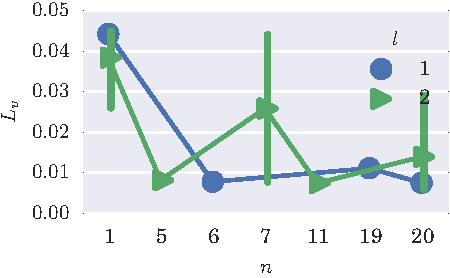
\includegraphics[]{figs/bo_sleep.pdf}
        \caption{PSG-ECG}
    \end{subfigure}%

\label{fig:bo}
\caption{Bayesian optimized validation loss} %todo: make tbls sentence case
\end{figure}
%todo: make figures centered by adding whitespace to the right



\section{Results and Discussion}
\label{sec:results}

The optimal RNN has some expectation of the typical series.
%
So, a `reconstruction error' is the difference between the test input and the output.
%
Therefore, the square of the reconstruction error can be used as an anomaly score \cite{Erfani2014}.
%
This section will show how the various calculations of error can be used to detect point anomalies \emph{as well as} discord anomalies introduced in \ref{this}.
%
However, the particular (objective) anomaly detection technique will not be discussed;
only the anomaly score, that could be used for such a technique, is presented.
%
Nonetheless, the argument is made for the ability of autoencoding RNNs to detect anomalies.


Although the order of the anomaly scores should not be important to the anomaly detection technique, sequences of error calculations can be made in two ways for a test series: 1) the MSE of a sliding window and 2) the squared error of every point in the test series where the whole sequence is input to the optimal RNN.
%
As discussed in Section \ref{this}, while the MSE from a sliding window can detect both point anomalies and discords, it is preferable not to have to specify a window size.
%
Ideally, high anomaly scores for points close together signal a discord while a lone high anomaly score signals a point anomaly.
%
But both types of caclulations are evaluated in this discussion.


Error calculations are presented graphically in Figure \ref{fig:err} for each series.
%
In the top pane, a portion of the input series is shown with an anomaly.
%
While the focus is on the anomaly, enough normal data is shown for subjective comparison.
%
The extremes of the ordinate are the extremes of all the input.
%
The lower panes show series of squared error, $\epsilon$, where each pane is associated with a sliding window size.
%
The window size is represented by a highlighted vertical span in the error plot as well as a corresponding box in the input series plot to give a sense of scale to anomaly relative to the window.
%
Sliding a window over the test series that caclulates its MSE generates the error series (calculation type 1).
%
The locations of the MSE points correspond with the center of the sliding window.
%
However, error plots with just a vertical line as a `window' are just individual squared errors (calculation type 2).
%
Furthermore, a kernel density estimate for all the errors (including ones outside the plot) is plotted (vertically) on the ordinate.
%
The highest 5 percentile and the maximum of (all) the errors are marked on the ordinate also.


The maximum, the kernel density estimate, and the 5 percentile mark give a summary of the errors.
%
Together, with the error plot, the efficacy of the RNN in distinguishing anomalies can be evaluated;
%
normal data should correspond to the bulk of the error calculations while anomalies should correspond to extreme high values.


It should be noted that as the window size is increased, fractionally less points are included in the, normal, 95 percentile (and vice versa).
%
The kernel desnity estimate might change significantly accordingly.


What follows is a discussion of the ability of the (optimal) RNN to detect anomalies referencing subfigures of Figure \ref{fig:err}.



\noindent {\bfseries{spikes}}

This series can be considered discrete with a point anomaly.
%
The errors were discrete as well with the anomaly region taking on specific values.
%
Clearly, the anomalies are distinguised in all error calculations.


\noindent {\bfseries{sine}}

This series tests discord because no single point is anomalous.
%
For the windowed errors, the anomalous and normal regions are distinguished by a range of values for each.
%
But, there was a transition region with errors higher or lower than the anomalous region.
%
In the point error plot, the extreme values correspond to extreme values in the test plot.
%
So, given these results, the windowed error can be more attributed to the extreme values of the test series than to its anomalous behaviour.
%
In any case the RNN found a tight expectation for typical values.


\noindent {\bfseries{power}}

The power series normally shows a daily demand profile over a five-day work week.
%
The windowed error distribution has a long tail because high errors were given to normal areas of test series (not shown within the plot).
%
In fact, the first windowed error plot does not contain the highest error unlike the second windowed error plot.
%
Nonetheless, both windowed errors distinguished the anomalous region.
%
But, obviously, the point errors can not be used to detect the anomalous region.


\noindent {\bfseries{ECG}}

The ECG is a challenging series because, while there is a repeating element, the element does not precicely have the same period.
%
There is also noise in the signal that has to be distinguished from its significant features.

In the point error plot, the most prominent values correspond to points on the test series that are simply lower than a baseline.
%
The same cannot be said about the error plot with the smallest window;
%
although the areas with extreme values are the most prominent, areas that have different behavior, but not extreme in value, are distinguished as well.
%
This window size was chosen to be about the size of the repeating unit since the effect on the error is diluted for larger windows.
%
Still, the argument can be made that the larger windows captured the anomalous region's behavior, as opposed to just its extreme values, because a significant portion of the error corresponding to the anomalous region lies within the 95 percentile (and hence within the normal range of fluctuations for normal data). %weak :S


\noindent {\bfseries{PSG-ECG}}

In this ECG, the point errors do not real much about the anomalous region becuase every spike in the error plot plot corresponds to a normal spike in the ECG, normal or otherwise.
%
However, the anomalous region is clearly detected in both windowed error plots. Again the error is well beyond the normal range of error fluctuations.


%todo: get validation error plts
%todo: can add linear trend
%todo: the figs should accompany the text. split the figs


\begin{figure}[t!] %todo: i think gmu wants all figs at the top
    \centering
  
  \begin{subfigure}[t]{\textwidth}
        \centering
        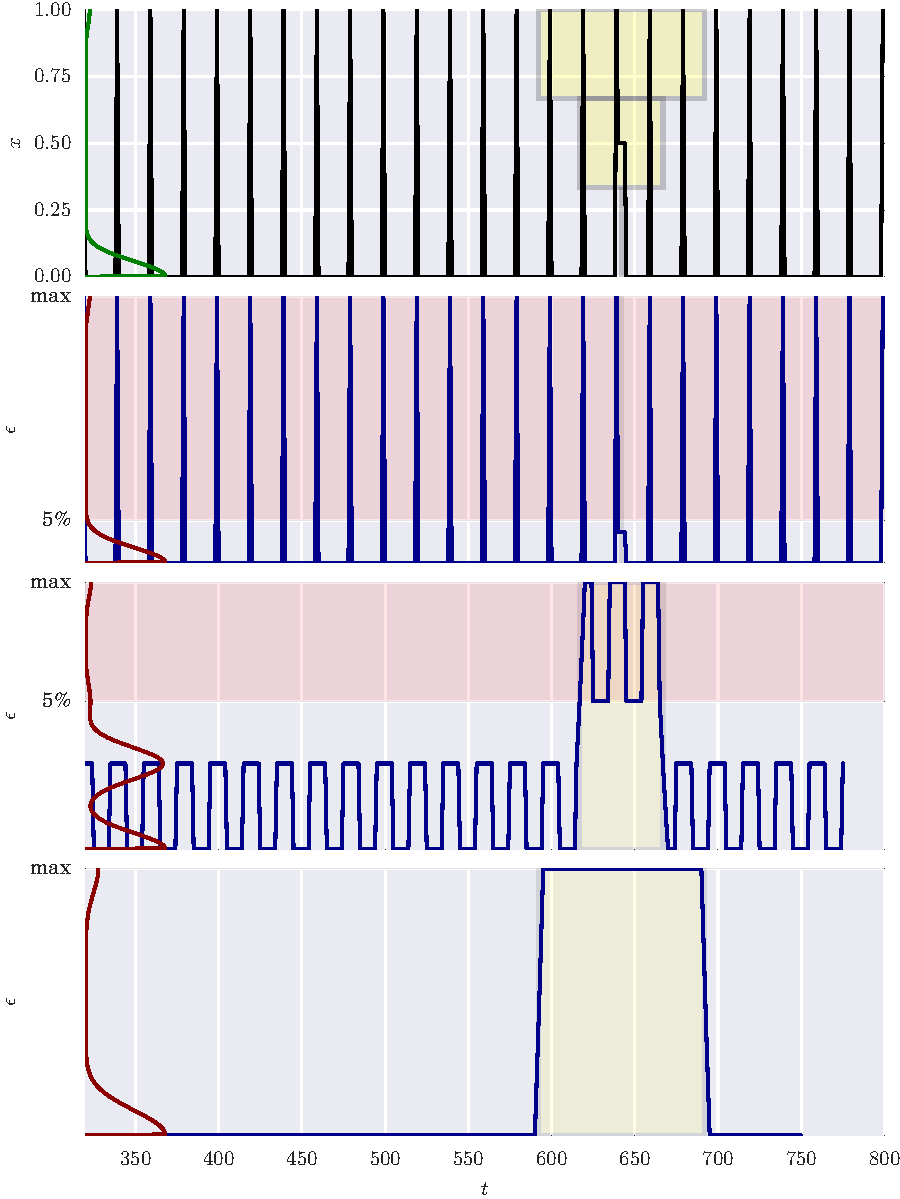
\includegraphics[]{figs/er_spike.pdf}
        \caption{spikes}
    \end{subfigure}%


\end{figure}
\begin{figure}
    \ContinuedFloat 
  
    \begin{subfigure}[t]{\textwidth}
        \centering
        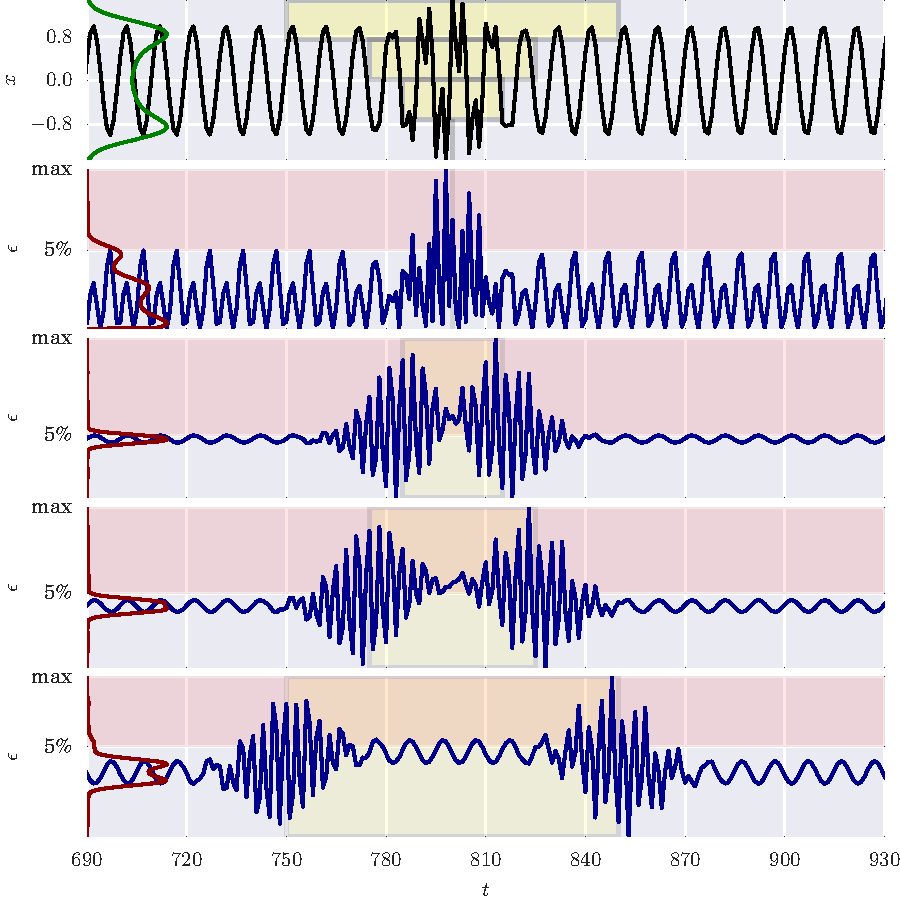
\includegraphics[]{figs/er_sin.pdf}
        \caption{sine}
    \end{subfigure}%

\end{figure}
\begin{figure}
    \ContinuedFloat 

    \begin{subfigure}[t]{\textwidth} 
        \centering
        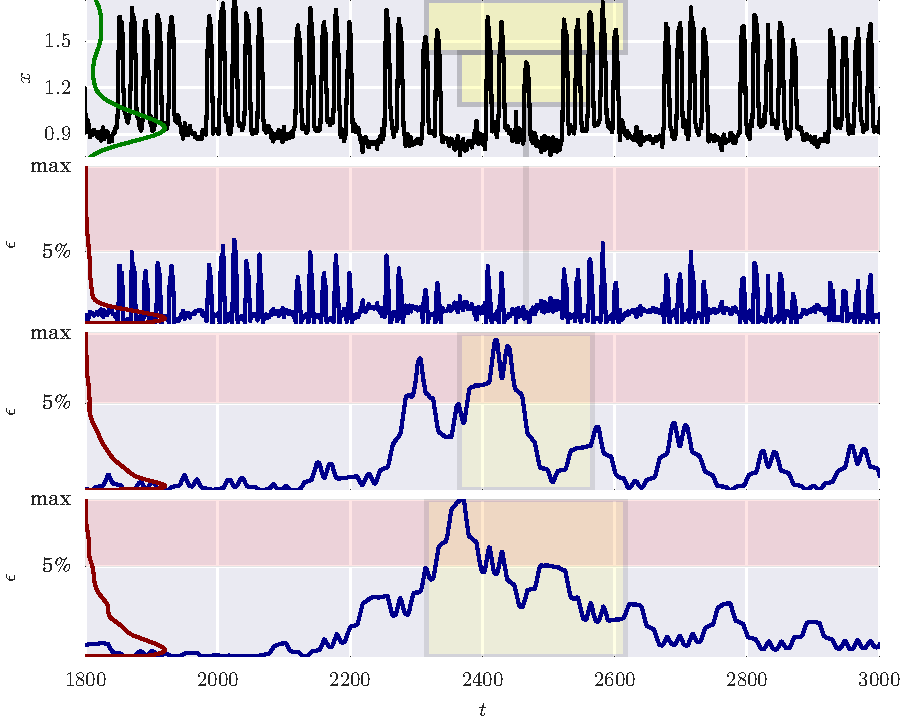
\includegraphics[]{figs/er_power.pdf}
        \caption{power}
    \end{subfigure}%

\end{figure}
\begin{figure}
    \ContinuedFloat 

    \begin{subfigure}[t]{\textwidth} 
        \centering
        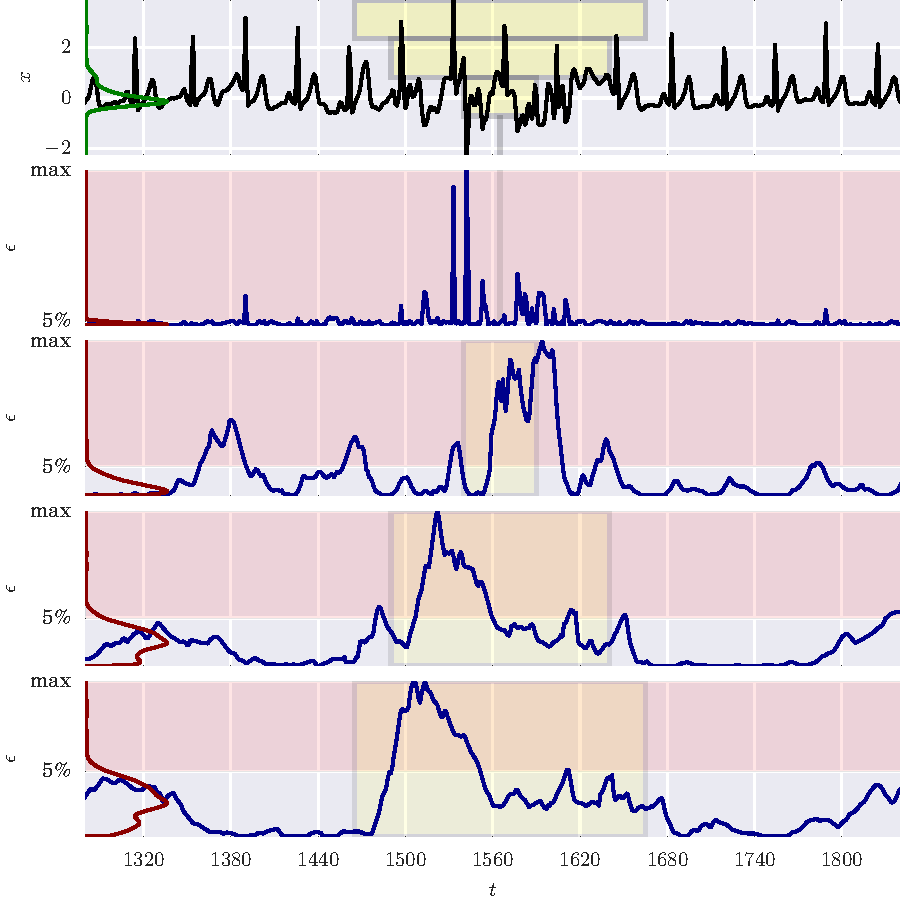
\includegraphics[]{figs/er_ecg.pdf}
        \caption{ECG}
    \end{subfigure}%

\end{figure}
\begin{figure}
    \ContinuedFloat

    \begin{subfigure}[t]{\textwidth} 
        \centering
        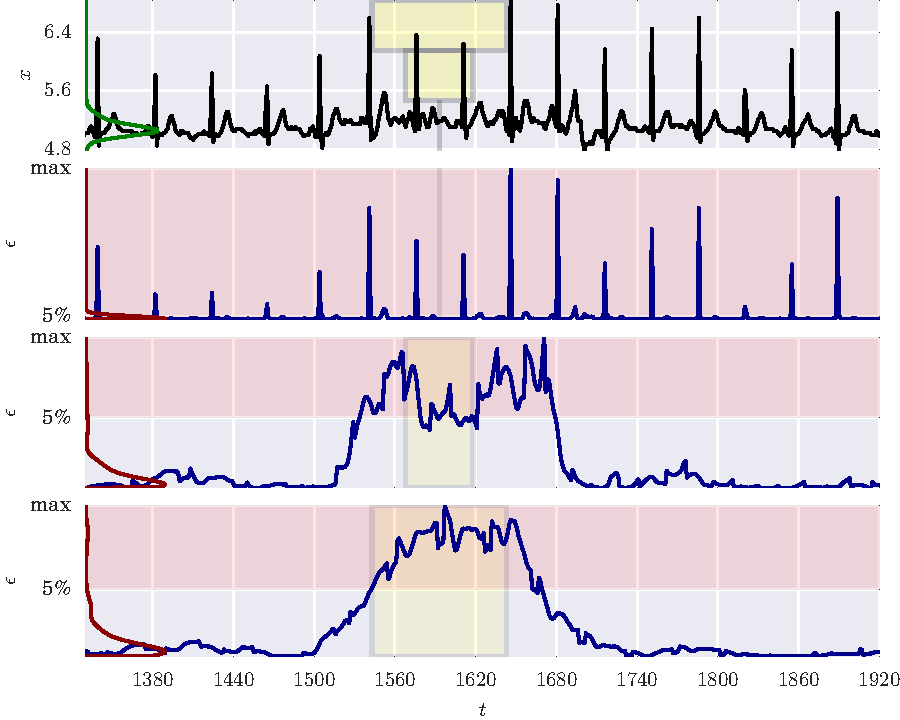
\includegraphics[]{figs/er_sleep.pdf}
        \caption{PSG-ECG}
    \end{subfigure}%

\label{fig:err}
\caption{Anomaly scores of series} 
%todo: make tbls captions sentence case but no period
\end{figure}



%todo . theano implememtation particularly slow suspected
%todo. include tbls and probabilitydfs in repo in final

%%% Local Variables:
%%% mode: latex
%%% TeX-master: "thesis"
%%% End:
